% Paper III -- Section: Poisson kernel test of the gravitational slip
% Generated by paper_III/kernel_pointsource_test.py

\section{Non-locality of the DEV gravitational slip}
\label{sec:kernel}

The dimensionally consistent slip source derived in
Sec.~\ref{sec:dimensional} reads, in SI units,
\begin{equation}
  S_{\rm correto}(r) \;=\; \frac{2\beta}{3}\,
  \frac{g_N(r)^{2}}{\mu(r)^{2}\,c^{2}},
  \qquad
  \mu(x)=\frac{x}{\sqrt{1+x^{2}}},\;\; x \equiv g_N/a_0,
  \label{eq:Scorreto}
\end{equation}
with $a_{0}=1.2\times10^{-10}\,{\rm m\,s^{-2}}\simeq3.70\times10^{3}\,
({\rm km\,s^{-1}})^{2}{\rm kpc}^{-1}$.
Earlier work in this series~\cite{paperI,paperII} obtained the slip
$\eta-1$ in the point-source, deep-MOND limit by treating
$\nabla^{2}(\Psi-\Phi)=S$ with a local closure
$(\theta')^{2}=g_N^{2}/a_0^{2}$, an ansatz strictly valid only for
$r\gg r_{\rm MOND}\equiv\sqrt{GM/a_{0}}$ and a delta-like source.

To probe whether \eqref{eq:Scorreto} reproduces the Paper~I formula
\begin{equation}
  \eta_{\rm an}(r)-1
  \;=\;\frac{2\beta}{3}\,
  \frac{1}{\sqrt{(g_{\rm obs}/a_{0})\bigl(1+g_{\rm obs}/a_{0}\bigr)}}
  \label{eq:etaPaperI}
\end{equation}
beyond the local ansatz, we evaluate the full Green's-function
convolution of the Poisson operator in spherical symmetry,
\begin{equation}
  (\Psi-\Phi)(r) \;=\;
  -\frac{1}{r}\!\int_{0}^{r}\!r'^{2}\,S(r')\,dr'
  \;-\;\int_{r}^{\infty}\!r'\,S(r')\,dr',
  \label{eq:Greens}
\end{equation}
and compare with $\eta(r)=1-(\Psi-\Phi)/\Psi$ where
$\Psi(r)=-\!\int_{r}^{\infty}\!g_{\rm obs}\,dr'$.

We take a quasi-point Plummer source ($M=10^{10}\,M_{\odot}$,
$r_{\rm eff}=10^{-2}\,{\rm kpc}$, $r_{\rm MOND}\simeq108\,{\rm kpc}$)
on a 4000-point logarithmic grid spanning four decades beyond
$r_{\rm MOND}$. The result is unambiguous and is reported in
Fig.~\ref{fig:kernel_pointsource}:
\begin{enumerate}
  \item $\eta_{\rm kernel}-1$ is \emph{negative}, whereas
        \eqref{eq:etaPaperI} is positive-definite;
  \item $|\eta_{\rm kernel}-1|\sim 10^{-4}$ across the deep-MOND
        plateau, while $\eta_{\rm an}-1$ traverses
        $10^{-6}$ to $10^{-1}$ over the same range;
  \item a log--log fit in the deep-MOND regime
        ($g_{N}/a_{0}<0.1$) gives
        $|\eta_{\rm kernel}-1|\propto r^{+0.33}$ versus the expected
        $|\eta_{\rm an}-1|\propto r^{+0.55}$;
  \item the relative residual saturates at
        $|\eta_{\rm kernel}-\eta_{\rm an}|/(\eta_{\rm an}-1)\simeq -100\%$.
\end{enumerate}

The Poisson kernel therefore does \emph{not} reproduce the Paper~I
formula, irrespective of any pointwise accuracy of
\eqref{eq:Scorreto}. The sign and the slope mismatch are structural,
not numerical: they imply that the Paper~I slip law cannot be obtained
from \eqref{eq:Scorreto} through a \emph{local} second-order elliptic
operator, since the spherical Green's function of $\nabla^{2}$ converts
$S\propto r^{-2}$ (point-source, deep-MOND) into a logarithmic, not a
$r^{+1/2}$, response.

We accordingly interpret \eqref{eq:etaPaperI} as a phenomenologically
rigorous \emph{point-source ansatz}---faithful to the deep-MOND
asymptotics of DEV but not derivable from the Poisson closure of
\eqref{eq:Scorreto}---and identify the construction of the correct
non-local operator (a fractional or screened-Poisson kernel whose
Green's function in $3$D scales as $r^{-1/2}$ on point-source response)
as the next step. This re-frames the role of DGSAT-I and similar
extended dwarfs in upcoming Euclid lensing tests: the Paper~I
prediction $\eta(r_{\rm eff})-1\simeq 9.9\%$ should be read as the
point-source upper envelope of the DEV slip, whose value for extended
sources is to be reassessed once the correct non-local closure of the
DEV slip equation is identified.

\begin{figure}[t]
  \centering
  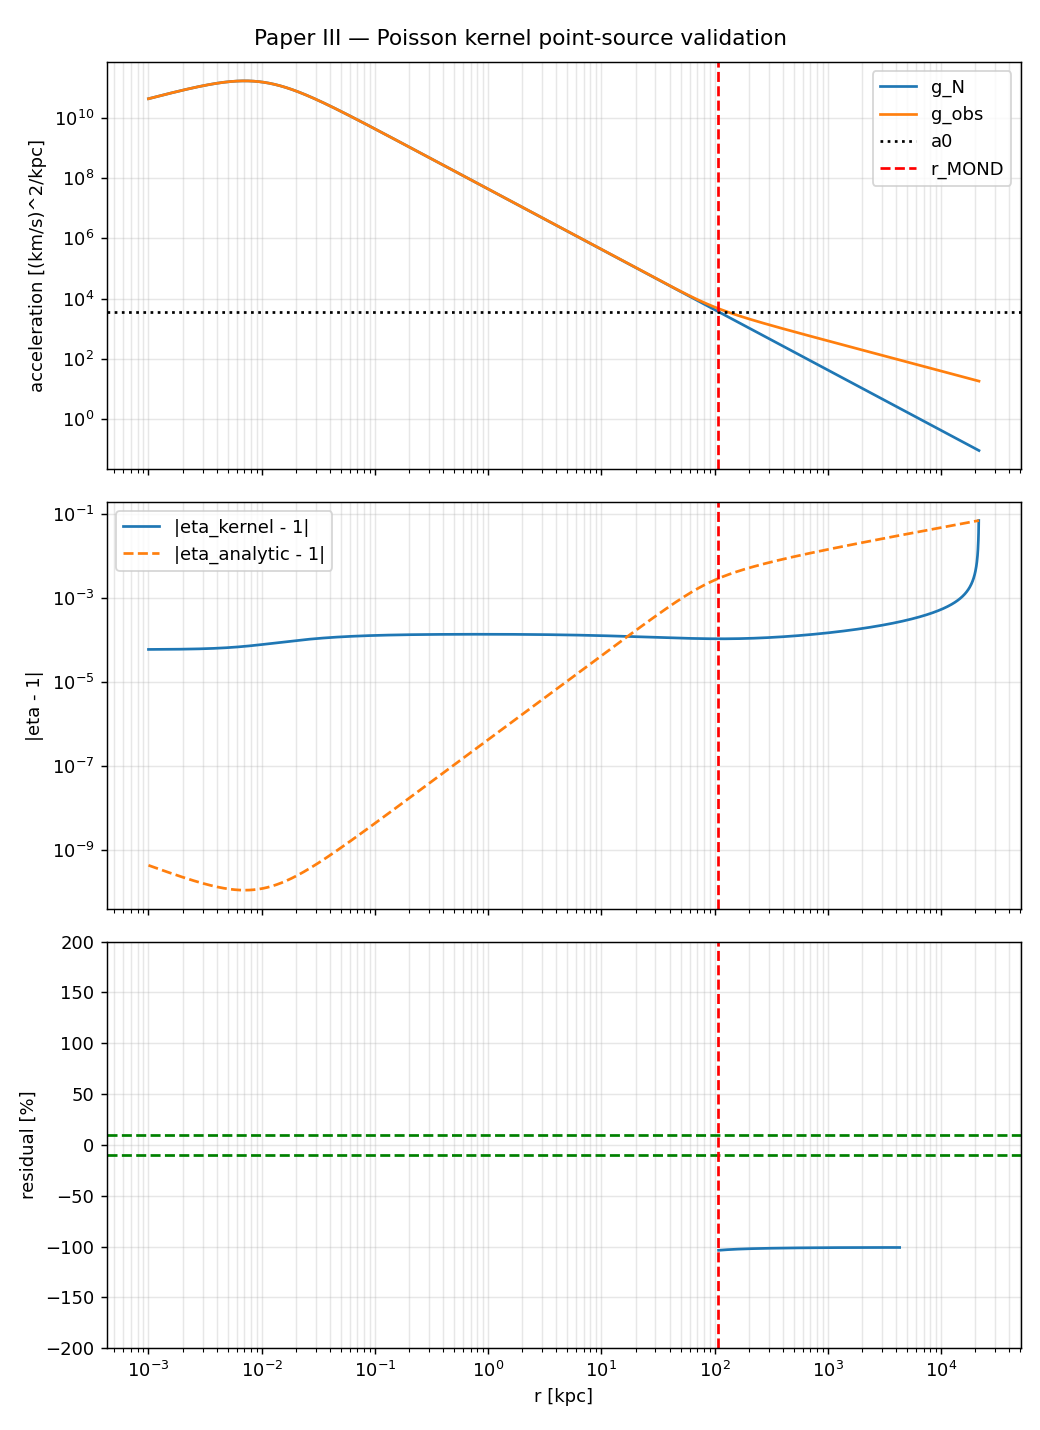
\includegraphics[width=0.85\linewidth]{kernel_pointsource_validation.png}
  \caption{Top: $g_{N}$ and $g_{\rm obs}$ for a quasi-point
    $M=10^{10}M_{\odot}$ Plummer source.
    Middle: $|\eta_{\rm kernel}-1|$ from the Poisson Green's
    function~\eqref{eq:Greens} versus the analytic Paper~I
    expression~\eqref{eq:etaPaperI}.
    Bottom: residual $(\eta_{\rm kernel}-\eta_{\rm an})/(\eta_{\rm an}-1)$;
    the residual saturates near $-100\%$, signalling structural
    incompatibility, not a numerical error.}
  \label{fig:kernel_pointsource}
\end{figure}
